\section{Results}
\label{sec:results}

The numerical results for the problem described in Section \ref{sec:requests} are reported in the following.

\begin{figure}[H]
    \centering
    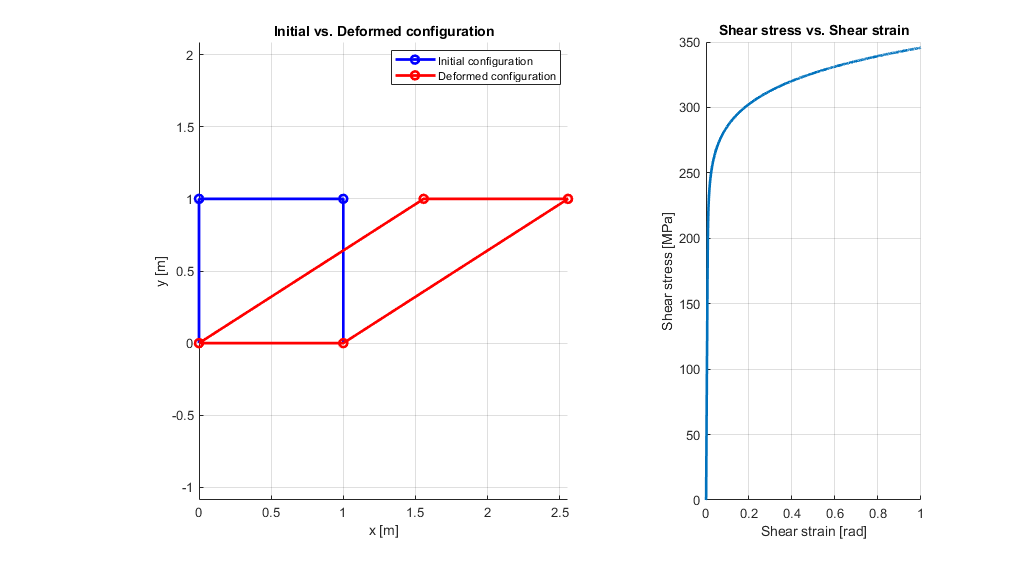
\includegraphics[width=\textwidth]{./img/stress_vs_strain.png}
    \caption{Shear stress $\sigma_{12}$ as function of $\gamma$.}
    \label{fig:stress_vs_strain}
\end{figure}

In Figure \ref{fig:stress_vs_strain} the curve $\sigma_{12}(\gamma)$ is plotted.

As we can see, in the first part of the curve the material behaves linearly.
Here the material is in the elastic region, and the slope of the curve is constant.

After this first linear region, the material starts to behave non-linearly.
This is due to the fact that the material has reached the yield strength, and the material starts to deform plastically.
The slope of the curve is not constant anymore, and the material starts to harden.


\subsection{Different elastic constitutive equations}

In the requests of the problem (Section \ref{sec:requests}), we were asked to compare the following two different elastic constitutive equations:

\begin{align}
    \dot{\sigma} & = C : \dot{\varepsilon} \\
    \sigma^{oT}  & = C: D
\end{align}

In our code we implemented the possibility to chose between the two constitutive equations for the elastic predictor step.
However, we weren't sure how to proceed with the implementation of the Trusdell objective rate inside the Radial Return algorithm.


\subsection{Loading and unloading cycles}

In order to better understand the behavior of the material after the yield  strength is reached, we can try to simulate a loading and unloading cycle.

In particular, considering the same problem as before, we can simulate the following loading and unloading cycle:

\begin{table}[H]
    \centering
    \begin{tabular}{|c|c|c|}
        \hline
        \textbf{Step} & \textbf{Loading direction} & \textbf{Stop condition} \\
        \hline
        1             & Positive                   & $\gamma = 0.03$         \\
        2             & Negative                   & $\sigma_{12} = 0$       \\
        3             & Positive                   & $\gamma = 0.05$         \\
        4             & Negative                   & $\gamma = -0.01$        \\
        5             & Positive                   & $\gamma = 0.1$          \\
        \hline
    \end{tabular}
    \caption{Loading and unloading cycle stages and relative conditions.}
    \label{tab:loading_unloading_cycle}
\end{table}

From the conditions above, the shear stress-strain curve in Figure \ref{fig:loading_unloading_cycle} is obtained.

\begin{figure}[H]
    \centering
    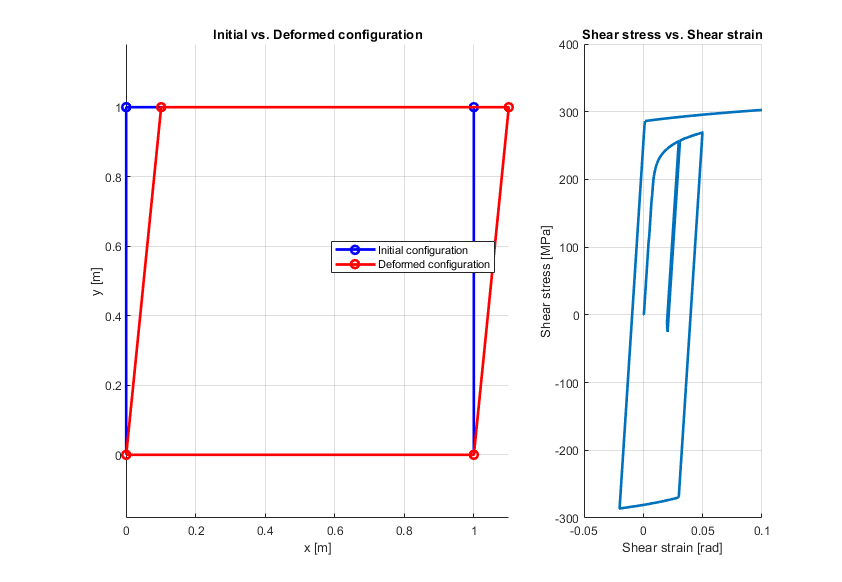
\includegraphics[width=\textwidth]{./img/loading_unloading_cycle.png}
    \caption{Shear stress $\sigma_{12}$ as function of $\gamma$ for the loading and unloading cycle.}
    \label{fig:loading_unloading_cycle}
\end{figure}

It's easy to see how only the elastic deformation is reversible and can be recovered after the unloading stage.
Instead, the plastic deformation is not recovered even after a complete unloading of the material.

This behavior can be explained by the model used to describe the material, where in the elastic region molecular structures are deformed elastically and the binding between atoms act as springs.
On the other hand, in the plastic region, the material undergoes permanent deformation due to the breaking of atomic bonds and the formation of new bonds in different positions (plane slip).

Among the files attached to this report, a video is provided to show the relationship between the deformed configuration of the structure and the stress-strain curve.

% , with a slope of $G = \frac{E}{2(1+\nu)}$ approximately (depending on the constitutive model choose based on Cauchy stress rate or Trusdell objective rate)